\documentclass[a4paper]{article}

%%%%%%%% CREATE DOCUMENT STRUCTURE %%%%%%%%
%% Language and font encoding
\usepackage[english]{babel}
% \usepackage[utf8x]{inputenc}
\usepackage[T1]{fontenc}
%\usepackage{algo}
\usepackage{algorithm}
\usepackage{algorithmic}
\usepackage{float}

%% Sets page size and margins
\usepackage[a4paper,top=3cm,bottom=2cm,left=2cm,right=2cm,marginparwidth=1.75cm]{geometry}

\bibliographystyle{plainurl}% the mandatory bibstyle

% %% Useful packages
\usepackage{amssymb}
\usepackage{algorithm}
% \usepackage{algorithmic}
\usepackage{amsmath}
\usepackage{amsthm}
\usepackage{graphicx}
\usepackage{multirow}
\usepackage{appendix}
\usepackage{stmaryrd}
\usepackage[super]{nth}
\usepackage[colorlinks=true, allcolors=blue]{hyperref}

\usepackage{caption}
\usepackage{subcaption}
\usepackage{sectsty}
\usepackage{apacite}
\usepackage{float}
\usepackage{titling} 
\usepackage{blindtext}
\usepackage{enumerate}
\usepackage{amsbsy}
\usepackage{makecell}
\usepackage[square,sort,comma,numbers]{natbib}
\usepackage[table, dvipsnames]{xcolor}
\usepackage[framemethod=tikz]{mdframed}
\definecolor{CB_pink}{HTML}{882255}
\definecolor{CB_green}{HTML}{117733}
\definecolor{CB_blue}{HTML}{332288}

% Packages for code formatting
\usepackage{listings} % For formatted code
\usepackage{minted}   % For syntax-highlighted code (requires -shell-escape)
\usepackage{verbatim} % For simple verbatim text

% Packages for trees formatting
\usepackage{tikz}
\usetikzlibrary{shapes.geometric, arrows}

\newtheoremstyle{remarksStyle}% 〈name〉
    {1.5em}% 〈Space above〉1
    {3pt}% 〈Space below 〉1
    {\rmfamily}% 〈Body font 〉
    {}% 〈Indent amount 〉2
    {\rmfamily\bfseries\itshape}% 〈Theorem head font 〉
    {:}% 〈Punctuation after theorem head 〉
    {0.5em}% 〈Space after theorem head 〉3
    {}% 〈Theorem head spec (can be left empty, meaning ‘normal’ )〉
\theoremstyle{remarksStyle}
\newtheorem*{observation}{Observation}
\newtheorem*{remark}{Remark}
\newtheorem*{definition}{Definition}

\newtheoremstyle{questionStyle}% 〈name〉
    {1.5em}% 〈Space above〉1
    {3pt}% 〈Space below 〉1
    {\rmfamily}% 〈Body font 〉
    {}% 〈Indent amount 〉2
    {\rmfamily\bfseries\color{CB_pink}}% 〈Theorem head font 〉
    {:}% 〈Punctuation after theorem head 〉
    {0.5em}% 〈Space after theorem head 〉3
    {}% 〈Theorem head spec (can be left empty, meaning ‘normal’ )〉
\theoremstyle{questionStyle}
\newtheorem{question}{Question}

\newtheoremstyle{answerStyle}% 〈name〉
    {3pt}% 〈Space above〉1
    {3pt}% 〈Space below 〉1
    {\rmfamily}% 〈Body font 〉
    {8pt}% 〈Indent amount 〉2
    {\rmfamily\bfseries\color{CB_green}}% 〈Theorem head font 〉
    {:}% 〈Punctuation after theorem head 〉
    {0.5em}% 〈Space after theorem head 〉3
    {}% 〈Theorem head spec (can be left empty, meaning ‘normal’ )〉
\theoremstyle{answerStyle}
\newtheorem{answer}{Answer}

\newmdenv[innerlinewidth=0.5pt, roundcorner=4pt,linecolor=CB_blue,innerleftmargin=6pt,
innerrightmargin=6pt,innertopmargin=6pt,innerbottommargin=6pt,backgroundcolor=Gray!15]{boxxed}


%%%%%%%% DOCUMENT %%%%%%%%
\begin{document}

%%%% Title Page
\begin{titlepage}

\newcommand{\HRule}{\rule{\linewidth}{0.5mm}}                           % horizontal line and its thickness
\center 
 
% University
\textsc{\LARGE Ben-Gurion University of the Negev}\\[1cm]

% Document info
\textsc{\Large Data Structures}\\[0.2cm]
\textsc{\large 202.1.1031}\\[1cm]                                       % Course Code
\HRule \\[0.8cm]
{ \huge \bfseries Assignment No. 1}\\[0.7cm]                                % Assignment
\HRule \\[2cm]
\large
\emph{Responsible staff members:}\\
{Prof. Paz Carmi} (carmip@bgu.ac.il)\\
Jules Zisser (zisserh@post.bgu.ac.il)\quad\quad Ilan Naiman (naimani@post.bgu.ac.il)\\[1.5cm]       
% Students info
% TODO fill out your names and IDs
\emph{Authors:}\\
John Doe (123456789)\quad Jane Doe (987654321)\\[1.5cm]
{\large Publication date: March 30th, 2025}\\
{\large Submission date: April 20th, 2025}\\[1cm]
{\large \it Update date: March 17th, 2025}\\[5cm]

\includegraphics[width=0.6\textwidth]{BGU-Icon.png}\\[1cm]  % University logo
\vfill 
\end{titlepage}
\newpage
\section{Submission Guidelines}
\begin{itemize}
    \item The submission is in pairs or individuals. We recommend working in pairs to encourage discussion and mutual inspiration.
    For the avoidance of doubt, if the assignment was submitted in pairs, all of the submitted answers should be the outcome of a joint work.
    \item Whether you submit as a pair or an individual, you must choose a group in the group assignment resource in Moodle.
    Groups created for individuals are of the form Assignment1\_s\_20, and groups for pairs are of the form Assignment1\_p\_100.
    \item Your submission should be a single pdf file (composed by LaTeX or any other word processor such as MS Word), and its name should be your group name (as chosen in Moodle), i.e., for the pair 17, the file name should be \verb!Assignment1_p_17.pdf!.
    \item Questions regarding the assignment should be asked in the dedicated forum in Moodle or during the office hours of the responsible staff members.
    The forum is intended to allow students to discuss the assignment. 
    The crew will answer questions in the forum when clarification is required in the pinned FAQ thread. 
    \item $\log{()}$ in the course is in base $2$, i.e., $\log_2{()}$ unless stated otherwise.
    \item A submission that does not include the integrity statement \textbf{\textcolor{Bittersweet}{will receive a score of 0}}.
\end{itemize}

\textbf{Before starting your work, read the following instructions carefully:}
\begin{itemize}
\item With each version of your work, submit it so that with each submission a larger part of your work is complete. This way, you won't lose major parts of your work due to a technical issue or unexpected circumstances.
\item DO NOT wait until the final hour for submitting your work, because there might be a power stoppage/computer issues/internet issues/Moodle issues/etc.
\item save a continuous backup of your work in some cloud platform, so that you can access it from any device if your computer decides to malfunction.
\item In case you work in pairs, both partners must verify that the work was submitted timely and fully. This way, you will prevent uncomfortable situations in cases of technical issues.
\end{itemize}


\newpage
\section{Integrity Statement}
Each of the students submitting this assignment must sign the following integrity statement:

\vspace{5ex}
\begin{boxxed}
\textcolor{CB_blue}{
We, \textbf{\textit{Dolev Rubin}}, ID number \textbf{\textit{319127379}}, and \textbf{\textit{Hila Zuckerman}}, ID number \textbf{\textit{212735450}} assert that the work we submitted is entirely our own.
We have not received any part from any other student in the class, nor did we give parts of it for others to use.
We realize that if my work is found to contain code that is not originally our own, a formal case will be opened against us with the BGU disciplinary committee.
}
\end{boxxed}

%\newpage
\vspace{1cm}

%%%% SECTIONS
\section{Complexity Hierarchy}
\begin{question} (20 points)
For each of the functions below place $f_{i}$ in the table in the correct place according to the following requirements:
\begin{itemize}
\item Functions $f_{i}$ and $f_{j}$ will be located on the same line if and if $f_{i}(n) \in \Theta(f_{j}(n))$  
\item For each function $f_{i}$ in line $k$ and $f_{j}$ in line $k+1$, $f_{i}(n) \in O(f_{j}(n))$
\end{itemize}
Your task is:
\begin{itemize}
    \item For each of two functions $f_{i}, f_{j}$ you have placed in the same line in the table show constants $c_1, c_2$ and $n_0$ suitable for the definition of $f_{i}(n) \in \Theta(f_{j}(n))$.
    \item For each two functions $f_{i}$ you have placed in line $k$ in the table and $f_{j}$ you have  placed in line $k+1$ show constants $c, n_0$ suitable for the definition of $f_{i}(n) \in O(f_{j}(n))$.
\end{itemize}

\begin{boxxed}
For example, for the following three functions:
\begin{enumerate}
    \item $f_{1}(n) = n^2 -10$
      \item $f_{2}(n) = 6$
    \item $f_{3}(n) = 22 n^2 + 10n$
\end{enumerate}
The table will look:
\begin{center}
\begin{tabular}{||c | c ||} 
 \hline
 line number & The functions \\ [0.5ex] 
 \hline\hline
 1 &  $f_{2}$ \\ 
 \hline
 2 &  $f_{1},f_{3}$\\ 
  \hline
\end{tabular}
\end{center}
\begin{itemize}
    \item $f_{2} \in \ O(f_{1}): \ 6 \leq c(n^2 -10)$ for $n \ge n_0 =4$ and $c=2$.
   \item  $f_{1} \in \ \Theta(f_{3}):$
      \begin{itemize}
          \item   $f_{1} \in \ O(f_{3}): \ n^2 -10 \leq c(n^2 -10)$ for $n \ge n_0 =1$ and $c=1$.
         \item $f_{1} \in \ \Omega(f_{3}): \ n^2 -10 \geq c(n^2 -10)$ for $n \ge n_0 =6$ and $c=\frac{1}{32}$.
     \end{itemize} 
\end{itemize} 
\textbf{Notice, since there are two functions in Line 2, it is enough to compare $f_{2}$ to only one of them.}
\end{boxxed}

\begin{enumerate}
    \item $f_{1}(n) = 1$
    \item $f_{2}(n) = 1034$
    \item $f_{3}(n) = n^{2}$
    \item $f_{4}(n) = n^{n}$
    \item $f_{5}(n) = 2^{n + \log n - 10}$
    \item $f_{6}(n) = 2^{(2^{n})}$
    \item $f_{7}(n) = 2^{n}$
    \item $f_{8}(n) = \log{(4^{n}*n^{8})}$
    \item $f_{9}(n) = \log{(n^{\frac{1}{3}})}$
    \item $f_{10}(n) = \frac{6n^2}{8} - 10$
   
\end{enumerate}


\begin{answer}
    Fill in the table below (\textbf{The Proof elaboration in this question is according to the example given above}):
\end{answer}

\begin{center}
\begin{tabular}{||c | c ||} 
 \hline
 line number & The functions \\ [0.5ex] 
 \hline\hline
 1 & $f_1, f_2$ \\ 
 \hline
 2 & $f_9$ \\
 \hline
 3 & $ f_8 $\\
 \hline
 4 &  $ f_3, f_10$\\
 \hline
 5 & $ f_7 $\\
 \hline
 6 & $ f_5 $\\
 \hline
 7 & $ f_4 $\\
 \hline
 8 & $ f_6 $\\
 \hline
 9 & \\
 \hline
  10 & \\
 \hline
\end{tabular}
\end{center}
\end{question}

\begin{boxxed}
\begin{itemize}
   \item  $f_{1} \in \ \Theta(f_{2}):$
      \begin{itemize}
          \item   $f_{1} \in \ O(f_{2}): \ 1 \leq c(1034)$ for $n \ge n_0 =1$ and $c=1$.
         \item $f_{1} \in \ \Omega(f_{2}): \ 1 \geq c(1034)$ for $n \ge n_0 =1$ and $c=\frac{1}{10000}$.
     \end{itemize} 

    \item $f_{1} \in \ O(f_{9}): \ 1 \leq c\log(n^\frac{1}{3}) = \frac{c}{3} \log(n) $ for $n \ge n_0 =8$ and $c=1$.

    \item $f_{9} \in \ O(f_{8}): \ \log(n^\frac{1}{3}) \leq c \cdot \log(4^n \cdot n^8) = c \cdot n \log(4) + 8 \log(n) = c \cdot (2n + 8\log(n)) $ for $n \ge n_0 =2$ and $c=1$.

    \item $f_{8} \in \ O(f_{3}): \ \log(4^n \cdot n^8) = 2n + 8\log(n) \leq cn^2 $ for $n \ge n_0 =8$ and $c=1$.
    
    \item  $f_{10} \in \ \Theta(f_{3}):$
      \begin{itemize}
          \item   $f_{10} \in \ O(f_{3}): \ \frac{6n^2}{8} - 10 \leq cn^2 $ for $n \ge n_0 =1$ and $c=1$.
         \item $f_{10} \in \ \Omega(f_{3}): \ \frac{6n^2}{8} - 10 \geq cn^2$ for $n \ge n_0 =10$ and $c=\frac{1}{8}$.
     \end{itemize} 

    \item $f_{3} \in \ O(f_{7}): \ n^2 \leq c \cdot 2^n $ for $n \ge n_0 =5$ and $c=1$.
    
    \item $f_{7} \in \ O(f_{5}): \ 2^n \leq c \cdot 2^{n + \log(n) -10} = c \cdot 2^{n-10} \cdot 2^{log(n)} = n \cdot 2^{n-10} $ for $n \ge n_0 =1$ and $c=2^{11}$.

    \item $f_{5} \in \ O(f_{4}): \ 2^{n + \log(n) -10} \leq c \cdot n^n $ for $n \ge n_0 =10$ and $c=1$.

    \item $f_{4} \in \ O(f_{6}): \ n^n \leq c \cdot 2^{(2^n)} $ for $n \ge n_0 =5$ and $c=3$.
    

\end{itemize} 

\end{boxxed}


\newpage

\section {Properties of asymptotic bounds}
\begin{question} (25 points) \label{q2}
Let $f(n)$ and $g(n)$ be asymptotically positive functions.

\begin{definition}
    We say that a function $f: \mathbb{N} \to \mathbb{N}$ is \textbf{unbounded increasing monotone function} if:
    \begin{enumerate}
        \item for all $x,y$:
        \[\text{\hspace{6cm}}x < y \iff f(x) < f(y) \text{\hspace{1.4cm} ($\iff$ stands for if and only if)}\]

        
        \item for all constant $M\in \mathbb{R}^+$ there is $n_0 \in \mathbb{N}$ such that for all $n > n_0$:
        \[f(n) > M\]
    \end{enumerate}
\end{definition}

\begin{boxxed}
    \textcolor{CB_blue}{
    The logarithm function is an \textbf{unbounded increasing monotone function} defined for $x > 0$.}
\end{boxxed}

\begin{boxxed}
    \textcolor{CB_blue}{
    In conjectures \ref{q2:log} and \ref{q2:exp} you can assume that for all constant $c > 0$, there is $x_0 > 0$ such that for all $x > x_0$: \[c < \frac{x}{\log x}\]}
\end{boxxed}

\vspace{1ex}
\textbf{Prove each of the following conjectures:}

\begin{enumerate}
    \item (4 points) $n > \log n $ for all $n \in \mathbb{N}$
    \item (2 points) Reflexivity: $f(n) \in \Theta(f(n))$
    \item (4 points) Transitivity: If $f(n) \in \Theta(g(n))$ and $g(n) \in \Theta(h(n))$ then $f(n) \in \Theta(h(n))$
    \item (3 points) Transpose Symmetry: $f(n) \in O(g(n)) \iff g(n) \in \Omega(f(n))$
    \item (4 points) For all $f(n) > 1$ and $g(n) > 1$ two \textbf{\textcolor{Bittersweet}{unbounded increasing monotone functions}} such that $f(n) \in \Omega(g(n))$, imply \[\log (f(n)) \in \Omega(\log (g(n)))\]

    \item (4 points) \label{q2:log} For all constant $k \ge 1$ and for all constant $1 > \varepsilon > 0$:
    \[ \log^k (n) \in O (n^\varepsilon) \]
    \item (4 points) \label{q2:exp} For all constant $k \in \mathbb{N}$ and for all constant $\varepsilon > 0$ :
    \[n^k \in O( (1 + \varepsilon)^n)\]
\end{enumerate}
\end{question}

\begin{answer}
\item 
\section*{1. \( n > \log n \) for all \( n \in N \) }

We know that $n < 2^n$ for all $n \in N$, then: $\log(n) < log(2^n) = n \cdot \log(2) = n$

\section*{2. Reflexivity: \( f(n) \in \Theta(f(n)) \) }

By the definition of \(\Theta\)-notation, \( f(n) \in \Theta(f(n)) \) if there exist constants \( c_1, c_2 > 0 \) and \( n_0 \) such that:

\[
c_1 f(n) \leq f(n) \leq c_2 f(n) \quad \forall n \geq n_0.
\]

By choosing \( c_1 = 1 \) and \( c_2 = 1 \), the inequality holds in all cases, proving reflexivity.

\section*{3. Transitivity: If \( f(n) \in \Theta(g(n)) \) and \( g(n) \in \Theta(h(n)) \), then \( f(n) \in \Theta(h(n)) \)}

By the definition of $\Theta$:

\[
c_1 g(n) \leq f(n) \leq c_2 g(n),
\]

\[
d_1 h(n) \leq g(n) \leq d_2 h(n).
\]

Now we will multiply the equation by the relevant constant on each side:

\[
(c_1 d_1) h(n) \leq f(n) \leq (c_2 d_2) h(n).
\]

Since \( c_1 d_1 \) and \( c_2 d_2 \) are positive constants, \( f(n) \in \Theta(h(n)) \).

\section*{4. Transpose Symmetry: \( f(n) \in O(g(n)) \iff g(n) \in \Omega(f(n)) \)}

By the definition of Big-O:

\[
f(n) \leq c g(n) \quad \text{for a constant } c > 0 \text{ and sufficiently large } n.
\]

Rewriting:

\[
g(n) \geq \frac{1}{c} f(n),
\]

which is the definition of \( g(n) \in \Omega(f(n)) \), proving the transpose symmetry. 

\section*{5. If \( f(n) \in \Omega(g(n)) \) for increasing monotone functions, then \( \log f(n) \in \Omega(\log g(n)) \)}

Since \( f(n) \in \Omega(g(n)) \), there exist constants \( c > 0 \) and \( n_0 \) such that:

\[
f(n) \geq c g(n), \quad \forall n \geq n_0.
\]

Taking logarithms:

\[
\log f(n) \geq \log (c g(n)) = \log c + \log g(n).
\]

Since \( \log c \) is a constant, we have:

\[
\log f(n) \in \Omega(\log g(n)).
\]

\section*{6. \( \log^k(n) \in O(n^\epsilon) \) for constants \( k \geq 1 \) and \( 1 > \epsilon > 0 \) }

?

\section*{7. \( n^k \in O((1+\epsilon)^n) \) for constants \( k \) and \( \epsilon > 0 \) }
?
\end{answer}

\newpage

\section {Recurrence Examples}
\begin{question} (15 points)
Find and prove an asymptotic tight bound $\Theta$ for $T(n)$ in each of the following recurrences. Assume that $T(c) = c$ for $c \le 4$.
\begin{enumerate}
    \item $T(n) = 4T(\frac{n}{2}) + n$
    \item $T(n) = T(\frac{3}{7}n) + 1$
    \item $T(n) = 6T(\frac{n}{2}) + n^4 \log{n}$
    \item $T(n) = 8T(\frac{n}{2}) + n^4 + 3n^3  \log{n} $
    \item $T(n) = T(\sqrt{n}) + n $
    
\end{enumerate}
\end{question}

\begin{answer}
\item
    \subsection*{1. \( T(n) = 4T(n/2) + n \)}
Using the Master Theorem, we compare with the recurrence form:
\[
T(n) = aT(n/b) + f(n),
\]
where \( a = 4 \), \( b = 2 \), and \( f(n) = n \).

We check the condition \( f(n) = O(n^c) \) where \( c = \log_b a = \log_2 4 = 2 \).
Since \( f(n) = O(n^1) \) and \( n^1 = O(n^2) \), Case 1 of the Master Theorem applies:
\[
T(n) = \Theta(n^2).
\]

\subsection*{2. \( T(n) = T(3n/7) + 1 \)}
This recurrence can be solved using the iterative method:
\begin{align*}
T(n) &= T(3n/7) + 1 \\
&= T(9n/49) + 1 + 1 \\
&= \dots \\
&= T(3^k n / 7^k) + k.
\end{align*}
Stopping when \( n = 1 \), we find \( k = \log_{7/3} n \), leading to:
\[
T(n) = \Theta(\log n).
\]

\subsection*{3. \( T(n) = 6T(n/2) + n^4 \log n \)}
Here, \( a = 6 \), \( b = 2 \), and \( f(n) = n^4 \log n \).
\[
c = \log_2 6 \approx 2.585.
\]
Since \( f(n) = n^4 \log n = \Omega(n^{4 - \epsilon}) \) for small \( \epsilon \), we use the Master Theorem’s Case 3 with the regularity condition, leading to:
\[
T(n) = \Theta(n^4 \log n).
\]

\subsection*{4. \( T(n) = 8T(n/2) + n^4 + 3n^3 \log n \)}
Here, \( a = 8 \), \( b = 2 \), and \( f(n) = n^4 + 3n^3 \log n \).
\[
c = \log_2 8 = 3.
\]
Since \( f(n) = n^4 + 3n^3 \log n = \Omega(n^{4-\epsilon}) \) for small \( \epsilon \), the dominating term is \( n^4 \). By the Master Theorem, Case 3 applies:
\[
T(n) = \Theta(n^4).
\]

\subsection*{5. \( T(n) = T(\sqrt{n}) + n \)}
Using the recursion tree method:
\begin{align*}
T(n) &= T(n^{1/2}) + n \\
&= T(n^{1/4}) + n^{1/2} + n \\
&= \dots \\
&= T(1) + n + n^{1/2} + n^{1/4} + \dots.
\end{align*}
The sum approximates to \( O(n) \), so we conclude:
\[
T(n) = \Theta(n).
\]

\end{answer}

\vspace{2cm}

\section{Time Complexity}
\begin{question} (10 points)
    
Find the time complexity of the following algorithms in terms of $\Theta$ (you are not required to prove this asymptotic bound).
You are expected to analyze the asymptotic tight bound of each line in the algorithms, as presented in class for the analysis of insertion sort. 
In addition, show the calculation of $T(n)$ as done in the lecture.
\end{question}


\begin{algorithm}[H]\caption{Search ($array[int], key$)}
 \begin{algorithmic}[1]
  \RETURN   Foo Search($array, key, 0, array.length -1$) 
  \end{algorithmic} 
\end{algorithm} 



\begin{algorithm}[H]
  \caption{Foo Search (array[int], key, left, right)}
  \begin{algorithmic}[1]
    \STATE $output \gets -1$ \quad \textit{// default value for not found}
    \STATE  $i \gets left - 1$
    \IF{left $\leq$ right}
       \FOR  {$j = left$  \textbf{to} $right - 1$ }
           \IF{$array[j] \leq array[right]$}
              \STATE $i \gets i+1$
              \STATE exchange $array[i]$ with $array[j]$
          \ENDIF
      \ENDFOR  
      \STATE exchange $array[i+1]$ with $array[right]$
      \IF{$array[i+1]  = key$}
          \STATE  $output \gets i+1$
      \ELSIF{$array[i+1] \leq key$}
         \STATE  $output \gets$  Foo Search($array, key, left, i$)
      \ELSE
          \STATE $output \gets$    Foo Search($array, key, i+2, right$)
      \ENDIF
    \ENDIF
    \RETURN output
  \end{algorithmic} 
\end{algorithm} 



\newpage

\begin{answer}
    Fill in the table and calculate the sum $T(n)$ below (do not fill in the grayed-out entries):
\begin{center}    
\begin{tabular}{||c | c | c | c ||}
 \hline
 Line number & \makecell{Number of times \\ the line is performed} & Cost of a single repetition & Total cost of this line \\ [0.5ex]
 \hline\hline
 1 & $\Theta(1)$ & $\Theta(1)$ & $\Theta (1)$  \\
 \hline
 2 & $\Theta(1)$ & $\Theta(1)$ & $\Theta (1)$  \\
 \hline
 3 & $\Theta(1)$ & $\Theta(1)$ & $\Theta (1)$  \\
  \hline
 4 & $\Theta(n)$ & $\Theta(1)$ & $\Theta (n)$  \\
   \hline
 5 & $\Theta(n)$ & $\Theta(1)$ & $\Theta (n)$  \\
  \hline
 6 & $\Theta(n)$ & $\Theta(1)$ & $\Theta (n)$  \\
    \hline
 7 & $\Theta(n)$ & $\Theta(1)$ & $\Theta (n)$  \\
 \hline
 8 & \cellcolor{Gray} & \cellcolor{Gray} & \cellcolor{Gray} \\
 \hline
 9 & \cellcolor{Gray} & \cellcolor{Gray} & \cellcolor{Gray} \\
 \hline
 10 & $\Theta(1)$ & $\Theta(1)$ & $\Theta (1)$  \\
 \hline
 11 & $\Theta(1)$ & $\Theta(1)$ & $\Theta (1)$  \\
 \hline
 12 & $\Theta(1)$ & $\Theta(1)$ & $\Theta (1)$  \\
 \hline
 13 & $\Theta(1)$ & $\Theta(1)$ & $\Theta (1)$  \\
 \hline
 14 & $\Theta(1)$ & $\Theta(1)$ & $\Theta (1)$  \\
 \hline
 15 & \cellcolor{Gray} & \cellcolor{Gray} & \cellcolor{Gray} \\
 \hline
 16 & $\Theta(1)$ & $\Theta(1)$ & $\Theta (1)$  \\
 \hline
 17 & \cellcolor{Gray} & \cellcolor{Gray} & \cellcolor{Gray} \\
 \hline
 18 & \cellcolor{Gray} & \cellcolor{Gray} & \cellcolor{Gray} \\
 \hline
 19 & $\Theta(1)$ & $\Theta(1)$ & $\Theta (1)$  \\
 \hline
 Total & \cellcolor{Gray} & \cellcolor{Gray} & $\Theta (n)$  \\
 \hline
\end{tabular}
\end{center}
\item In the worst case, the "right" element is always the smallest or largest element in the array, leading to a seperation of the array to 2 sub arrays of size 1, and $n - 1$. Which leads to the following time complexity formula:
\[ T(n) = T(n-1) + n \]
\item Proof by induction that $ T(n) \in \theta(n^2)$:
\item induction base: $n = 1$:
\item $ 0 \leq c_1 \cdot 1^2 \leq T(1) = 1 \leq c_2 \cdot 1^2$ so $ c_1 = 1, c_2 = 1$

\item Induction step

\item $T(n) = T(n - 1) - n = T(n-2) + n - 1 +n = T(n - 3) + n- 2 +2n-1 = ... = T(n-i) + i \cdot n - \sum_{k=1}^{i-1} k = T(n-i) + i \cdot n - \frac{i \cdot (i-1)}{2}$
\item We want to find the i that will bring us to T(1) - the stopping condition: $ i = n - 1 $.
\item $T(n) = T(1) + n^2 - n - \frac{n^2}{2} + n + \frac{n}{2} - 1= T(1) + \frac{n^2}{2} + \frac{n}{2} - 1= \theta(1) + \theta(n^2) + \theta(n) = \theta(n^2)$

\end{answer}

\newpage
\section{Algorithm Development}
\begin{question} (10 points)
\label{q5:a}
Describe in pseudo-code an efficient algorithm for solving the following problem, and analyze its running time and additional memory usage. The running time should be as asymptotically low as possible.
\\
\textbf{Notice:} In this question you can assume that there is a \textbf{fast initializing array} that allows initialization of $n$ cells in a constant time, that is, in $\Theta(1)$.
This stands in contradiction to the RAM model displayed in class (in which allocation of $n$ cells is done in $\Theta(1)$ and initialization of all cells is $\Theta(n)$), and can be assumed in questions \ref{q5:a} and \ref{q6} only.
\paragraph{Input:} Two unsorted arrays $A$ and $B$ of size $N\in \mathbb {N}$. The value of each element in the arrays is a natural number in the range $[0,2N]$.
\paragraph{Output:} The number of elements in Array $B$ that appear in Array $A$. 

\paragraph{Examples:} $ $
\vspace{0.5cm}

Input:
\begin{tabular}{|c || c | c  | c | c | c | c | c ||} 
 \hline
 A & 5 & 2 & 14 & 2 & 2 & 7 & 1  \\ 
 \hline
 B & 6 & 9 & 9 & 10 & 13 & 0 & 8\\
 \hline
\end{tabular}

\vspace{0.5cm}
Output: 0


\vspace{1cm}
Input:
\begin{tabular}{|c || c | c  | c | c | c | c | c ||} 
 \hline
 A & 5 & 9 & 7 & 2 & 2 & 7 & 7  \\ 
 \hline
 B & 6 & 9 & 9 & 10 & 7 & 13 & 8\\
 \hline
\end{tabular}

\vspace{0.5cm}
Output:  3 \hspace{1cm} (\textit{9 appears in $A$ and appears twice in $B$,  7 appears in $A$  and appears once in $B$})


\vspace{1cm}
Input:
\begin{tabular}{|c || c | c  | c | c | c | c | c ||} 
 \hline
 A & 6 & 9 & 9 & 10 & 7 & 13 & 8  \\ 
 \hline
 B & 5 & 9 & 7 & 2 & 2 & 7 & 7  \\ 
 \hline
\end{tabular}

\vspace{0.5cm}
Output:  4 \hspace{1cm} (\textit{9 appears in $A$ and appears once in $B$,  7 appears in $A$  and appears three times in $B$})










\end{question}

\vspace{0.5 cm}

\begin{answer}
    Pseudocode of the algorithm:
\begin{minted}{python}
def question_5(A, B):
    """
    This pseudocode uses an additional array to indicate in O(1) time
    whether a number is in array A. the algorithm then loops throw the
    numbers in array B in order to perform the counting.
    """
    mem_array = new Array[2N] # filled with zeros, takes O(1) time and O(N) space.
    for number in A: # runs N times, so this for loop is O(N) overall.
        mem_array[number] = 1 # done in O(1)

    counter = 0
    for num in B: # runs N times, so this for loop is O(N) overall.
        if mem_array[num] == 1: # done in O(1)
            counter = counter + 1

    return counter # overall, the function runs in O(N) + O(N) = O(n)
        
\end{minted}
\end{answer}

\vspace{0.75 cm}

\begin{question} \label{q6} (5 points)
Solve question \ref{q5:a}, where the value of each element in the arrays is a natural number in the range $[0,N^2]$ (instead of $[0, 2N]$).
\end{question}

\vspace{0.5 cm}

\begin{answer}
    Pseudocode of the algorithm:
\begin{minted}{python}
def question_6(A, B):
    """
    This pseudocode is sorting array A usgin merge sort, and then performs
    binary search on every element of array B to check if it exists in A.
    """
    # sort using merge sort, O(n*log(n)) time complexity and O(n) memory complexity
    sortedA = sort(A) 
    
    counter = 0
    # runs n times, so this for loop is O(n*log(n)) time complexity overall.
    for number in B: 
        # done in O(log(n)) time complexity
        if binary_search(sortedA, number) == true: 
            counter = counter + 1

    # overall, this function runs in O(n*log(n)) time complexity and O(n) memory complexity
    return counter 
        
\end{minted}
\end{answer}

\newpage
\section{AVL tree}
\begin{question} (5 points)
The following sequence of keys has been added to an AVL tree.
$< 5, \ 6, \ 12, \ 10, 8 >$. 
\end{question}
\begin{answer}
\item
\begin{center}
        \vtop{
            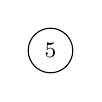
\begin{tikzpicture}[
                level 1/.style={sibling distance=20mm}, % Distance between sibling nodes
                level 2/.style={sibling distance=15mm}, % Distance between sibling nodes
                every node/.style={circle, draw, fill=white, font=\footnotesize} % Circle for nodes
                ]
                \node {5};
            \end{tikzpicture}
        }
    \end{center}
        \vspace{3mm}
        % Second TikZ picture (Node 6 with a right child) - aligned to top
    \begin{center}    
        \vtop{
            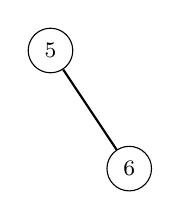
\begin{tikzpicture}[
                every node/.style={circle, draw, fill=white, font=\footnotesize}, % Circle for nodes
                level 1/.style={sibling distance=15mm}, % Adjust sibling distance
                edge from parent/.style={draw, thick} % Styling for edges
                ]
                \node {5}
                   child[shift={(1,0)}] {node {6}};
            \end{tikzpicture}
        }
    \end{center}
        \vspace{3mm}
    \begin{center}     
        % Third TikZ picture (Node 6 with two children) - aligned to top
        \vtop{
            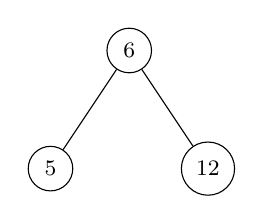
\begin{tikzpicture}[
                level 1/.style={sibling distance=20mm}, % Distance between sibling nodes
                level 2/.style={sibling distance=15mm}, % Distance between sibling nodes
                every node/.style={circle, draw, fill=white, font=\footnotesize} % Circle for nodes
                ]
                \node {6}
                child{node {5}}
                child{node {12}};
            \end{tikzpicture}
        }
    \end{center}
          \vspace{3mm}
    \begin{center}
        \vtop{
            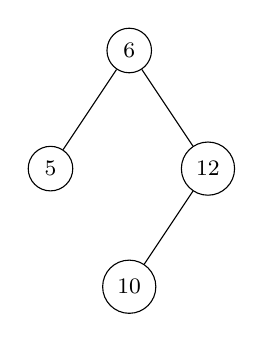
\begin{tikzpicture}[
            level 1/.style={sibling distance=20mm}, % Distance between sibling nodes
            level 2/.style={sibling distance=15mm}, % Distance between sibling nodes
            every node/.style={circle, draw, fill=white, font=\footnotesize} % Circle for nodes
            ]
        
                % Root node with only a right child positioned explicitly on the right
                \node {6}
                child{node {5}}
                child{node {12}
                    child[shift={(-1,0)}] {node {10}}};
        
            \end{tikzpicture}
        }
    \end{center}
         \vspace{3mm}
    \begin{center}
         \vtop{
             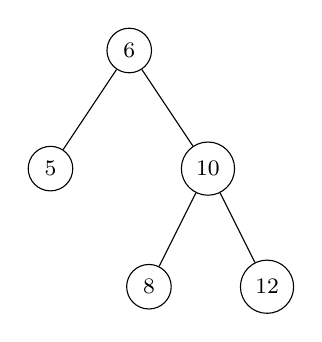
\begin{tikzpicture}[
            level 1/.style={sibling distance=20mm}, % Distance between sibling nodes
            level 2/.style={sibling distance=15mm}, % Distance between sibling nodes
            every node/.style={circle, draw, fill=white, font=\footnotesize} % Circle for nodes
            ]
        
                % Root node with only a right child positioned explicitly on the right
                \node {6}
                child{node {5}}
                child{node {10}
                    child{node {8}}
                    child{node {12}}
                    };
        
            \end{tikzpicture}
        }
    \end{center}

% \includegraphics[width=0.8\textwidth]{AAA.png}\\[1cm]
\end{answer}

\begin{question} (10 points)
Consider the following set $S$ of keys: $\{ 1,2,3,4,5,6,7 \} $
\end{question}
\begin{answer}
     Write an insertion sequence of the keys in $S$ that has \textbf{at least two rotations overall} and results in an AVL tree of  
         \begin{enumerate}
             \item[(i)] maximum height.
              \item[(ii)]  minimum height.
           \end{enumerate}


    \item[(i)] maximum height.
    $< 3, \ 2, \ 4, \ 5, \ 6, \ 7,\ 1>$

    \begin{center}
        \vtop{
            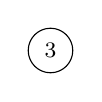
\begin{tikzpicture}[
                level 1/.style={sibling distance=20mm}, % Distance between sibling nodes
                level 2/.style={sibling distance=15mm}, % Distance between sibling nodes
                every node/.style={circle, draw, fill=white, font=\footnotesize} % Circle for nodes
                ]
                \node {3};
            \end{tikzpicture}
        }
    \end{center}
        \vspace{3mm}
        % Second TikZ picture (Node 6 with a right child) - aligned to top
    \begin{center}    
        \vtop{
            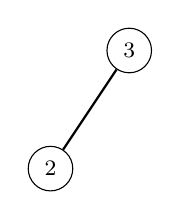
\begin{tikzpicture}[
                every node/.style={circle, draw, fill=white, font=\footnotesize}, % Circle for nodes
                level 1/.style={sibling distance=15mm}, % Adjust sibling distance
                edge from parent/.style={draw, thick} % Styling for edges
                ]
                \node {3}
                   child[shift={(-1,0)}] {node {2}};
            \end{tikzpicture}
        }
    \end{center}
        \vspace{3mm}
    \begin{center}     
        % Third TikZ picture (Node 6 with two children) - aligned to top
        \vtop{
            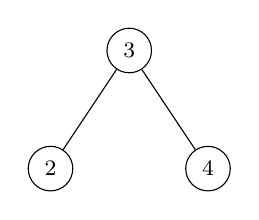
\begin{tikzpicture}[
                level 1/.style={sibling distance=20mm}, % Distance between sibling nodes
                level 2/.style={sibling distance=15mm}, % Distance between sibling nodes
                every node/.style={circle, draw, fill=white, font=\footnotesize} % Circle for nodes
                ]
                \node {3}
                child{node {2}}
                child{node {4}};
            \end{tikzpicture}
        }
    \end{center}
          \vspace{3mm}
    \begin{center}
        \vtop{
            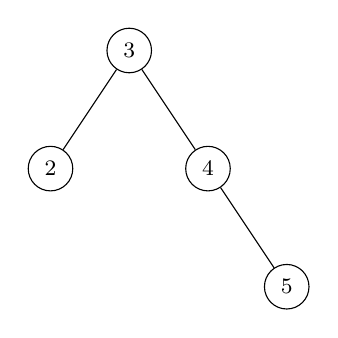
\begin{tikzpicture}[
            level 1/.style={sibling distance=20mm}, % Distance between sibling nodes
            level 2/.style={sibling distance=15mm}, % Distance between sibling nodes
            every node/.style={circle, draw, fill=white, font=\footnotesize} % Circle for nodes
            ]
        
                % Root node with only a right child positioned explicitly on the right
                \node {3}
                child{node {2}}
                child{node {4}
                    child[shift={(1,0)}] {node {5}}};
        
            \end{tikzpicture}
        }
    \end{center}
         \vspace{3mm}
         
    \begin{center}
    First rotation:
         \vtop{
         \vspace{3mm}
             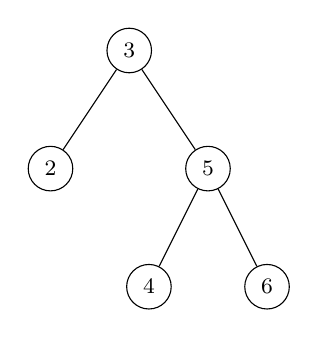
\begin{tikzpicture}[
            level 1/.style={sibling distance=20mm}, % Distance between sibling nodes
            level 2/.style={sibling distance=15mm}, % Distance between sibling nodes
            every node/.style={circle, draw, fill=white, font=\footnotesize} % Circle for nodes
            ]
        
                % Root node with only a right child positioned explicitly on the right
                \node {3}
                child{node {2}}
                child{node {5}
                    child{node {4}}
                    child{node {6}}};
        
            \end{tikzpicture}
        }
    \end{center}
    \vspace{3mm}

    \begin{center}
    Second rotation:
         \vtop{
         \vspace{3mm}
             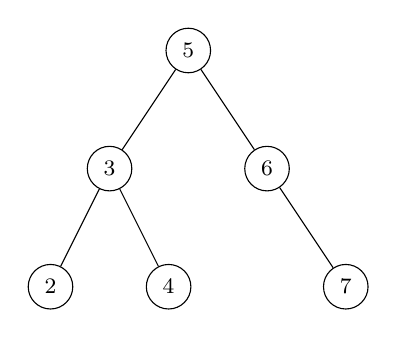
\begin{tikzpicture}[
            level 1/.style={sibling distance=20mm}, % Distance between sibling nodes
            level 2/.style={sibling distance=15mm}, % Distance between sibling nodes
            every node/.style={circle, draw, fill=white, font=\footnotesize} % Circle for nodes
            ]
        
                % Root node with only a right child positioned explicitly on the right
                \node {5}
                child{node {3}
                    child{node {2}}
                    child{node {4}}}
                child{node {6}
                    child[shift={(1,0)}] {node {7}}};
        
            \end{tikzpicture}
        }
    \end{center}

    \vspace{3mm}

    \begin{center}
         \vtop{
             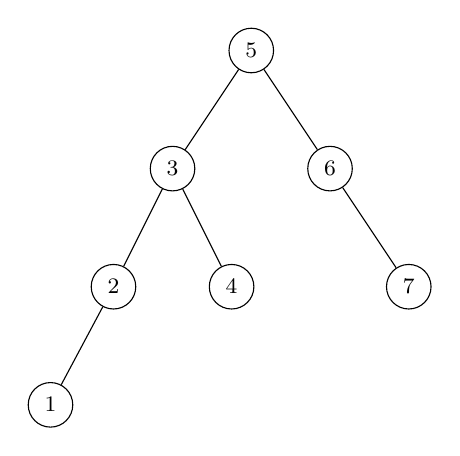
\begin{tikzpicture}[
            level 1/.style={sibling distance=20mm}, % Distance between sibling nodes
            level 2/.style={sibling distance=15mm}, % Distance between sibling nodes
            every node/.style={circle, draw, fill=white, font=\footnotesize} % Circle for nodes
            ]
        
                % Root node with only a right child positioned explicitly on the right
                \node {5}
                child{node {3}
                    child{node {2}
                    child[shift={(-0.8,0)}] {node {1}}}
                    child{node {4}}}
                child{node {6}
                    child[shift={(1,0)}] {node {7}}};
        
            \end{tikzpicture}
        }
    \end{center}
    
    \item[(ii)]  minimum height.
    $< 2, \ 1, \ 3, \ 4, \ 6, \ 5,\ 7>$

    \begin{center}
        \vtop{
            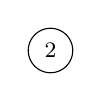
\begin{tikzpicture}[
                level 1/.style={sibling distance=20mm}, % Distance between sibling nodes
                level 2/.style={sibling distance=15mm}, % Distance between sibling nodes
                every node/.style={circle, draw, fill=white, font=\footnotesize} % Circle for nodes
                ]
                \node {2};
            \end{tikzpicture}
        }
    \end{center}
        \vspace{3mm}
        % Second TikZ picture (Node 6 with a right child) - aligned to top
    \begin{center}    
        \vtop{
            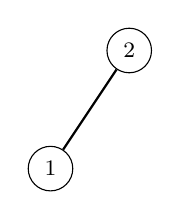
\begin{tikzpicture}[
                every node/.style={circle, draw, fill=white, font=\footnotesize}, % Circle for nodes
                level 1/.style={sibling distance=15mm}, % Adjust sibling distance
                edge from parent/.style={draw, thick} % Styling for edges
                ]
                \node {2}
                   child[shift={(-1,0)}] {node {1}};
            \end{tikzpicture}
        }
    \end{center}
        \vspace{3mm}
    \begin{center}     
        % Third TikZ picture (Node 6 with two children) - aligned to top
        \vtop{
            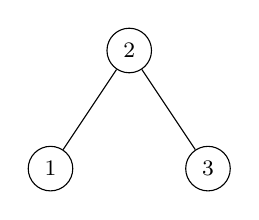
\begin{tikzpicture}[
                level 1/.style={sibling distance=20mm}, % Distance between sibling nodes
                level 2/.style={sibling distance=15mm}, % Distance between sibling nodes
                every node/.style={circle, draw, fill=white, font=\footnotesize} % Circle for nodes
                ]
                \node {2}
                child{node {1}}
                child{node {3}};
            \end{tikzpicture}
        }
    \end{center}
          \vspace{3mm}
    \begin{center}
        \vtop{
            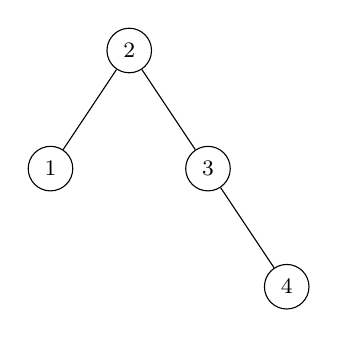
\begin{tikzpicture}[
            level 1/.style={sibling distance=20mm}, % Distance between sibling nodes
            level 2/.style={sibling distance=15mm}, % Distance between sibling nodes
            every node/.style={circle, draw, fill=white, font=\footnotesize} % Circle for nodes
            ]
        
                % Root node with only a right child positioned explicitly on the right
                \node {2}
                child{node {1}}
                child{node {3}
                    child[shift={(1,0)}] {node {4}}};
        
            \end{tikzpicture}
        }
    \end{center}
    \vspace{1mm}
         
    \begin{center}
    First rotation:
         \vtop{
         \vspace{1mm}
             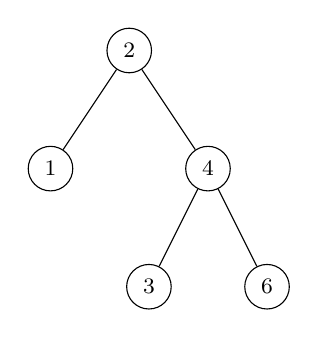
\begin{tikzpicture}[
            level 1/.style={sibling distance=20mm}, % Distance between sibling nodes
            level 2/.style={sibling distance=15mm}, % Distance between sibling nodes
            every node/.style={circle, draw, fill=white, font=\footnotesize} % Circle for nodes
            ]
        
                % Root node with only a right child positioned explicitly on the right
                \node {2}
                child{node {1}}
                child{node {4}
                    child{node {3}}
                    child{node {6}}};
        
            \end{tikzpicture}
        }
    \end{center}
    \vspace{1mm}
    \begin{center}
    Second rotation:
         \vtop{
         \vspace{1mm}
             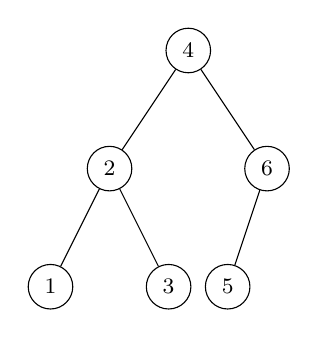
\begin{tikzpicture}[
            level 1/.style={sibling distance=20mm}, % Distance between sibling nodes
            level 2/.style={sibling distance=15mm}, % Distance between sibling nodes
            every node/.style={circle, draw, fill=white, font=\footnotesize} % Circle for nodes
            ]
        
                % Root node with only a right child positioned explicitly on the right
                \node {4}
                child{node {2}
                    child{node {1}}
                    child{node {3}}}
                child{node {6}
                    child[shift={(-0.5,0)}] {node {5}}};
        
            \end{tikzpicture}
        }
    \end{center}

    \vspace{3mm}

    \begin{center}
         \vtop{
             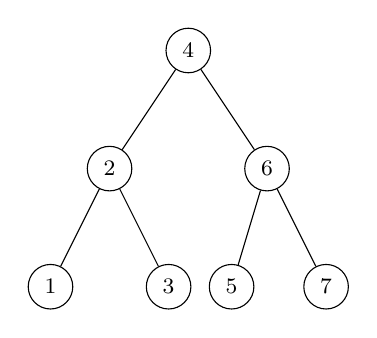
\begin{tikzpicture}[
            level 1/.style={sibling distance=20mm}, % Distance between sibling nodes
            level 2/.style={sibling distance=15mm}, % Distance between sibling nodes
            every node/.style={circle, draw, fill=white, font=\footnotesize} % Circle for nodes
            ]
        
                % Root node with only a right child positioned explicitly on the right
                \node {4}
                child{node {2}
                    child{node {1}}
                    child{node {3}}}
                child{node {6}
                    child[shift={(0.3,0)}] {node {5}}
                    child{node {7}}};
        
            \end{tikzpicture}
        }
    \end{center}
    
\end{answer}




\end{document}